Dans ce chapitre, un exemple de mise en œuvre du système de type décrit dans le
chapitre~\ref{cha:qualifs} et implanté dans le chapitre~\ref{cha:implem}.

\section{Linux}

Le noyau Linux, abordé dans le chapitre~\ref{cha:os}, est un noyau de système
d'exploitation développé depuis le début des années 90 et ``figure de proue'' du
mouvement open-source. Au départ écrit par Linus Torvalds sur son ordinateur
personnel, il a au fil des années était porté sur de nombreuses architectures et
s'est enrichi de nombreux pilotes de périphériques. En 20XX, son code source
comporte 8.8 millions de lignes de code (en grande majorité du C) dont 55\% de
pilotes.

% TODO fix le XX
% TODO mettre à jour

Même si le noyau est monolithique (la majeure partie des traitements s'effectue
au sein d'un même fichier objet), les sous-systèmes sont indépendants. C'est ce
qui permet d'écrire des pilotes de périphériques et des modules.

\section{GNU C}

Linux est écrit dans le langage C, mais pas sa version normalisée. Il utilise le
dialecte GNU C qui est celui que supporte GCC.

Pour traduire ce dialecte, il a été nécessaire d'adapter \texttt{c2newspeak}. La
principale particularité est la notation \texttt{\_\_attribute\_\_((...))} qui
peut décorer les déclarations de fonctions, de variables ou de types. De
nouvelles fonctionnalités sont aussi présentes.

Par exemple, il est possible de manipuler des étiquettes de première classe : si
\texttt{lbl:} est présent avant une instruction, on peut capturer l'adresse de
celle-ci avec \texttt{void *p = \&\&lbl} et y sauter indirectement avec
\texttt{goto *p}.

Une autre fonctionnalité est le concept d'instruction-expression :
\texttt{(\{bloc\})}) est une expression, dont la valeur est celle de la dernière
expression évaluée lors de \texttt{i}.

Les attributs, quant à eux, rentrent dans trois catégories :

\begin{itemize}
  \item les annotations de compilation ; par exemple, \texttt{used} désactive
    l'avertissement ``cette variable n'est pas utilisée ''.

  \item les optimisations ; par exemple, les objets marqués \texttt{hot} sont
    groupés de telle manière qu'ils se retrouvent en cache ensemble.

  \item les annotations de bas niveau ; par exemple, \texttt{aligned(n)}
    spécifie qu'un objet doit être aligné sur au moins \texttt{n} bits.
\end{itemize}

Dans notre cas, toutes ces annotations peuvent être ignorées.

\section{Configuration}

Pour que le code noyau soit compilable, il est nécessaire de définir certaines
macros. En particulier, le système de configuration de Linux utilise des macros
nommées \texttt{CONFIG\_*} pour inclure ou non certaines fonctionnalités. Il a
donc fallu faire un choix ; nous avons choisi la configuration par défaut. Pour
analyser des morceaux plus importants du noyau, il faudrait définir un fichier
de configuration plus important.

\section{Appels systèmes sous Linux}

Dans cette section, nous allons voir comment ces mécanismes sont implantés dans
le noyau Linux. Une description plus détaillée pourra être trouvée dans
\cite{UnderstandingTheLinuxKernel}, ou pour le cas de la mémoire virtuelle,
\cite{LinuxVMM}.

Deux rings sont utilisés : en \ring{0}, le code noyau et en \ring{3}, le code
utilisateur.

Une notion de tâche similaire à celle décrite dans la section~\ref{sec:taches}
existe : elles s'exécutent l'une après l'autre, le changement s'effectuant sur
interruptions.

Pour faire appel aux services du noyau, le code utilisateur doit faire appel à
des appels systèmes, qui sont des fonctions exécutées par le noyau. Chaque tâche
doit donc avoir deux piles : une pile ``utilisateur'' qui sert pour
l'application elle-même, et une pile ``noyau'' qui sert aux appels système.

\begin{figure} % fig:memmap {{{
\centering
\fbox{
  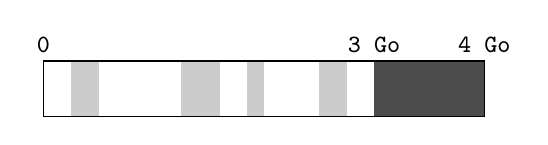
\begin{tikzpicture}
  [scale=0.7
  ,user/.style={fill=black!20}
  ,kernel/.style={fill=black!70}
  ]

  % Memory zone
  %
  % #1 - start
  % #2 - end
  % #3 - color
  \newcommand{\mzone}[3]{
    \path[#3] (#1,0) rectangle (#2,1);
  }

  % Address label
  %
  % #1 - x position
  % #2 - text
  \newcommand{\alabel}[2]{
    \path (#1,1) -- ++(0,0.3) node [pos=1] {\small \tt #2};

  }

  % exec
  \mzone{0.5}{1}{user}

  % lib
  \mzone{2.5}{3.2}{user}

  % stack
  \mzone{3.7}{4}{user}

  % stack
  \mzone{5}{5.5}{user}

  % kernel
  \mzone{6}{8}{kernel}

  % contour
  \draw (0,0) rectangle (8,1);

  \alabel{0}{0}
  \alabel{6}{3 Go}
  \alabel{8}{4 Go}

\end{tikzpicture}

}

\caption[Espace d'adressage d'un processus]{L'espace d'adressage d'un processus.
En gris clair, les zones accessibles à tous les niveaux de privilèges : code du
programme, bibliothèques, tas, pile. En gris foncé, la mémoire du noyau,
réservée au mode privilégié.}

\label{fig:memmap}
\end{figure}
% }}}

Grâce à la mémoire virtuelle, chaque processus possède sa propre vue de la
mémoire dans son espace d'adressage (figure~\ref{fig:memmap}), et donc chacun
un ensemble de tables de pages et une valeur de \crtrois associée. Au moment de
changer le processus en cours, l'ordonnanceur charge donc le \crtrois du nouveau
processus.

Les adresses basses (inférieures à \texttt{PAGE\_OFFSET} = 3 Gio =
\texttt{0xc0000000}) sont réservées à l'utilisateur. On y trouvera par exemple :

\begin{itemize}
\item le code du programme
\item les données du programmes (variables globales)
\item la pile utilisateur
\item le tas (mémoire allouée par \texttt{malloc} et fonctions similaires)
\item les bibliothèques partagées
\end{itemize}

Au dessus de \texttt{PAGE\_OFFSET}, se trouve la mémoire réservée au noyau.
Cette zone contient le code du noyau, les piles noyau des processus, etc.

\subsection{Appels système}
\label{sec:impl-syscall}

%TODO clarifier encore tout ça

Les programmes utilisateur s'exécutant en \ring{3}, ils ne peuvent pas
contenir d'instructions privilégiées, et donc ne peuvent pas accéder directement
au matériel (c'était le but !). Pour qu'ils puissent interagir avec le système
(afficher une sortie, écrire sur le disque...), le mécanisme des appels système
est nécessaire. Il s'agit d'une interface de haut niveau entre les \emph{rings}
3 et 0. Du point de vue du programmeur, il s'agit d'un ensemble de fonctions C
``magiques'' qui font appel au système d'exploitation pour effectuer des
opérations.

Voyons ce qui se passe derrière la magie apparente. Une explication plus
détaillée est disponible dans la documentation fournie par Intel
\cite{intelsys}.

\subsubsection{Dans la bibliothèque C}

Il y a bien une fonction \texttt{getpid} présente dans la bibliothèque C du
système. C'est la fonction qui est directement appelée par le programme. Cette
fonction commence par placer le numéro de l'appel système (noté
\texttt{\_\_NR\_getpid}, valant 20 ici) dans \eax, puis les arguments éventuels
dans les registres (\ebx, \ecx, \edx, \esi puis \edi). Une interruption
logicielle est ensuite déclenchée (\texttt{int 0x80}).

\subsubsection{Dans la routine de traitement d'interruption}

Étant donné la configuration du processeur\footnote{Il est impropre de dire que
le processeur est configuré --- tout dépend uniquement de l'état de certains
registres, ici la \emph{Global Descriptor Table} et les \emph{Interrupt
Descriptor Tables}.}, elle sera traitée en \ring{0}, à un point d'entrée
prédéfini (\texttt{arch/x86/kernel/entry\_32.S}, \texttt{ENTRY(system\_call)}).

\insertcode{entry-syscall.s}

L'exécution reprend donc en \ring{0}, avec dans \esp le pointeur de pile noyau
du processus. Les valeurs des registres ont été préservées, la macro
\texttt{SAVE\_ALL} les place sur la pile. Ensuite, à l'étiquette
\texttt{syscall\_call}, le numéro d'appel système (toujours dans \eax) sert
d'index dans le tableau de fonctions \texttt{sys\_call\_table}.


\subsubsection{Dans l'implantation de l'appel système}

Puisque les arguments sont en place sur la pile, comme dans le cas d'un appel de
fonction ``classique'', la convention d'appel \emph{cdecl} est respectée. La
fonction implantant l'appel système, nommée \texttt{sys\_getpid}, peut donc être
écrite en C.

On trouve cette fonction dans \texttt{kernel/timer.c} :

\insertcode{syscall-definition.c}

La macro \texttt{SYSCALL_DEFINE0} nomme la fonction \texttt{sys\_getpid}, et
définit entre autres des points d'entrée pour les fonctionnalités de débogage du
noyau. À la fin de la fonction, la valeur de retour est placée dans \eax,
conformément à la convention \emph{cdecl}.

\subsubsection{Retour vers le ring 3}

Au retour de la fonction, la valeur de retour est placée à la place de \eax là
où les registres ont été sauvegardés sur la pile noyau
(\texttt{PT\_EFLAGS(\%esp)}). L'instruction \texttt{iret} (derrière la macro
\texttt{INTERRUPT\_RETURN}) permet de restaurer les registres et de repasser en
mode utilisateur, juste après l'interruption. La fonction de la bibliothèque C
peut alors retourner au programme appelant.


\section{Bug}

On décrit le cas d'un pilote video qui contenait un bug de pointeur utilisateur.
Il est répertorié sur \url{http://freedesktop.org} en tant que bug \#29340. 

Pour changer de mode graphique, les pilotes de GPU peuvent supporter le
\emph{Kernel Mode Setting} (KMS).

Pour configurer un périphérique, l'utilisateur communique avec le pilote noyau
avec le mécanisme d'\emph{ioctls}\footnote{
  Ce nom vient de la fonction \texttt{ioctl()} pour
  \emph{Input/Output Control}.
}.
Ils sont similaires à des appels système, mais spécifique à un périphérique
particulier. Les fonctions implantant un \emph{ioctl} sont donc vulnérables à la
même classe d'attaques que les appels système, et donc doivent être écrits avec
une attention particulière.

Le code suivant est présent dans le pilote KMS pour les GPU AMD Radeon :

\begin{verbatim}
/* from drivers/gpu/drm/radeon/radeon_kms.c */
int radeon_info_ioctl(struct drm_device *dev,
                      void *data,
                      struct drm_file *filp) {
	struct radeon_device *rdev =
            dev->dev_private;
	struct drm_radeon_info *info;
	struct radeon_mode_info *minfo =
            &rdev->mode_info;
	uint32_t *value_ptr;
	uint32_t value;
	struct drm_crtc *crtc;
	int i, found;

	info = data;
	value_ptr = (uint32_t *)
            ((unsigned long)info->value);
	value = *value_ptr;
        [...]
}
\end{verbatim}

On peut voit que l'argument \texttt{data} est converti en un \texttt{struct
drm\_radeon\_info *}. Un pointeur \texttt{value\_ptr} est extrait de son champ
\texttt{value}, et finalement ce pointeur est déréferencé.

Cependant, l'argument \texttt{data} est un pointeur vers une structure (allouée
en espace noyau) du type suivant, dont les champs proviennent d'un appel
utilisateur de \texttt{ioctl()}.

\begin{verbatim}
/* from include/drm/radeon_drm.h */
struct drm_radeon_info {
  uint32_t    request;
  uint32_t    pad;
  uint64_t    value;
};
\end{verbatim}

Pour mettre ce problème en évidence, nous avons annoté la fonction
\texttt{radeon\_info\_ioctl} de telle manière que son second paramètre soit un
pointeur noyau vers une structure contenant un champ \qUser, \texttt{value}.
Ceci est possible puisqu'avant la traduction, on efface les types présents dans
le programme C. Ainsi, un pointeur ne peut pas être distingué d'un entier
transtypé en un pointeur. Avec cette configuration, nous obtenons une erreur de
type à la ligne 16.

L'intégralité de ce code peut être trouvée en annexe~\ref{cha:code-noyau}.

\begin{figure}
  \insertcode{radeon-git-mini.diff}

  \caption{Patch résolvant le problème de pointeur utilisateur.}
  \label{fig:linux-patch}
\end{figure}

% TODO décrire syntaxe unified diff

La bonne manière de faire a été publiée avec le numéro de \emph{commit}
\texttt{d8ab3557} (figure~\ref{fig:linux-patch}) (\texttt{DRM\_COPY\_FROM\_USER}
étant une simple macro pout \texttt{copy\_from\_user}). Dans ce cas, on
n'obtient pas d'erreur de typage.

% TODO et l'assembleur inline?

\section{Détails}

Pour utiliser notre système de types, plusieurs étapes sont nécessaires en plus
de traduire le noyau linux en \langname.

Afin de réaliser l'analyse, il faut annoter les sources pour créer un
environnement initial (via la variable \texttt{exttbl} décrite en
section~\ref{sec:ptrtype-archi}).

% TODO dire ce qu'on annote : les sources de pointeurs souillés

Ensuite, il faut réécrire les fonctions de manipulation de pointeurs fournies
par le noyau : \texttt{get\_user}, \texttt{put\_user},
\texttt{copy\_from\_user}, \texttt{copy\_to\_user}, etc. Leur implantation
revient à réaliser un test puis à faire la copie. À leur place on utilise les
primitives $\phxx{\uGet}$ et $\phxx{\uPut}$.

% TODO ... ou on ne met pas ces primitives là en tyspeak et on ajoute juste un
% bon type dans l'environnement initial

Enfin, on peut lancer l'inférence de type.
